\documentclass[journal]{IEEEtran}
\usepackage[a5paper, margin=10mm, onecolumn]{geometry}
\usepackage{amsmath, amssymb, mathtools}
\usepackage{graphicx}
\usepackage{gvv-book}
\usepackage{gvv}

\title{1.2.23 Matgeo}
\author{ai25btech11015 - M Sai Rithik}

\begin{document}
{\let\newpage\relax\maketitle}

\textbf{Question:} \\
Represent graphically a displacement of 40 km, $30^{\circ}$ west of south.

\textbf{Solution:} \\

We choose the coordinate axes such that:
\begin{itemize}
    \item $+x$ axis $\to$ East
    \item $+y$ axis $\to$ North
\end{itemize}

The given displacement has magnitude
\[
|\vec{D}| = 40 \ \text{km}
\]
and direction $30^{\circ}$ west of south.  

South corresponds to $270^{\circ}$, hence the angle from the positive $x$-axis is
\[
\theta = 270^{\circ} - 30^{\circ} = 240^{\circ}.
\]

The vector components are:
\[
D_x = 40 \cos 240^{\circ} = -20 \quad , \quad
D_y = 40 \sin 240^{\circ} = -20\sqrt{3}.
\]

Therefore,
\[
\vec{D} = -20\hat{i} - 20\sqrt{3}\hat{j}.
\]

Thus, the displacement vector is drawn from $(0,0)$ to
\[
(-20, \ -20\sqrt{3}).
\]

\begin{figure}[h!]
    \centering
    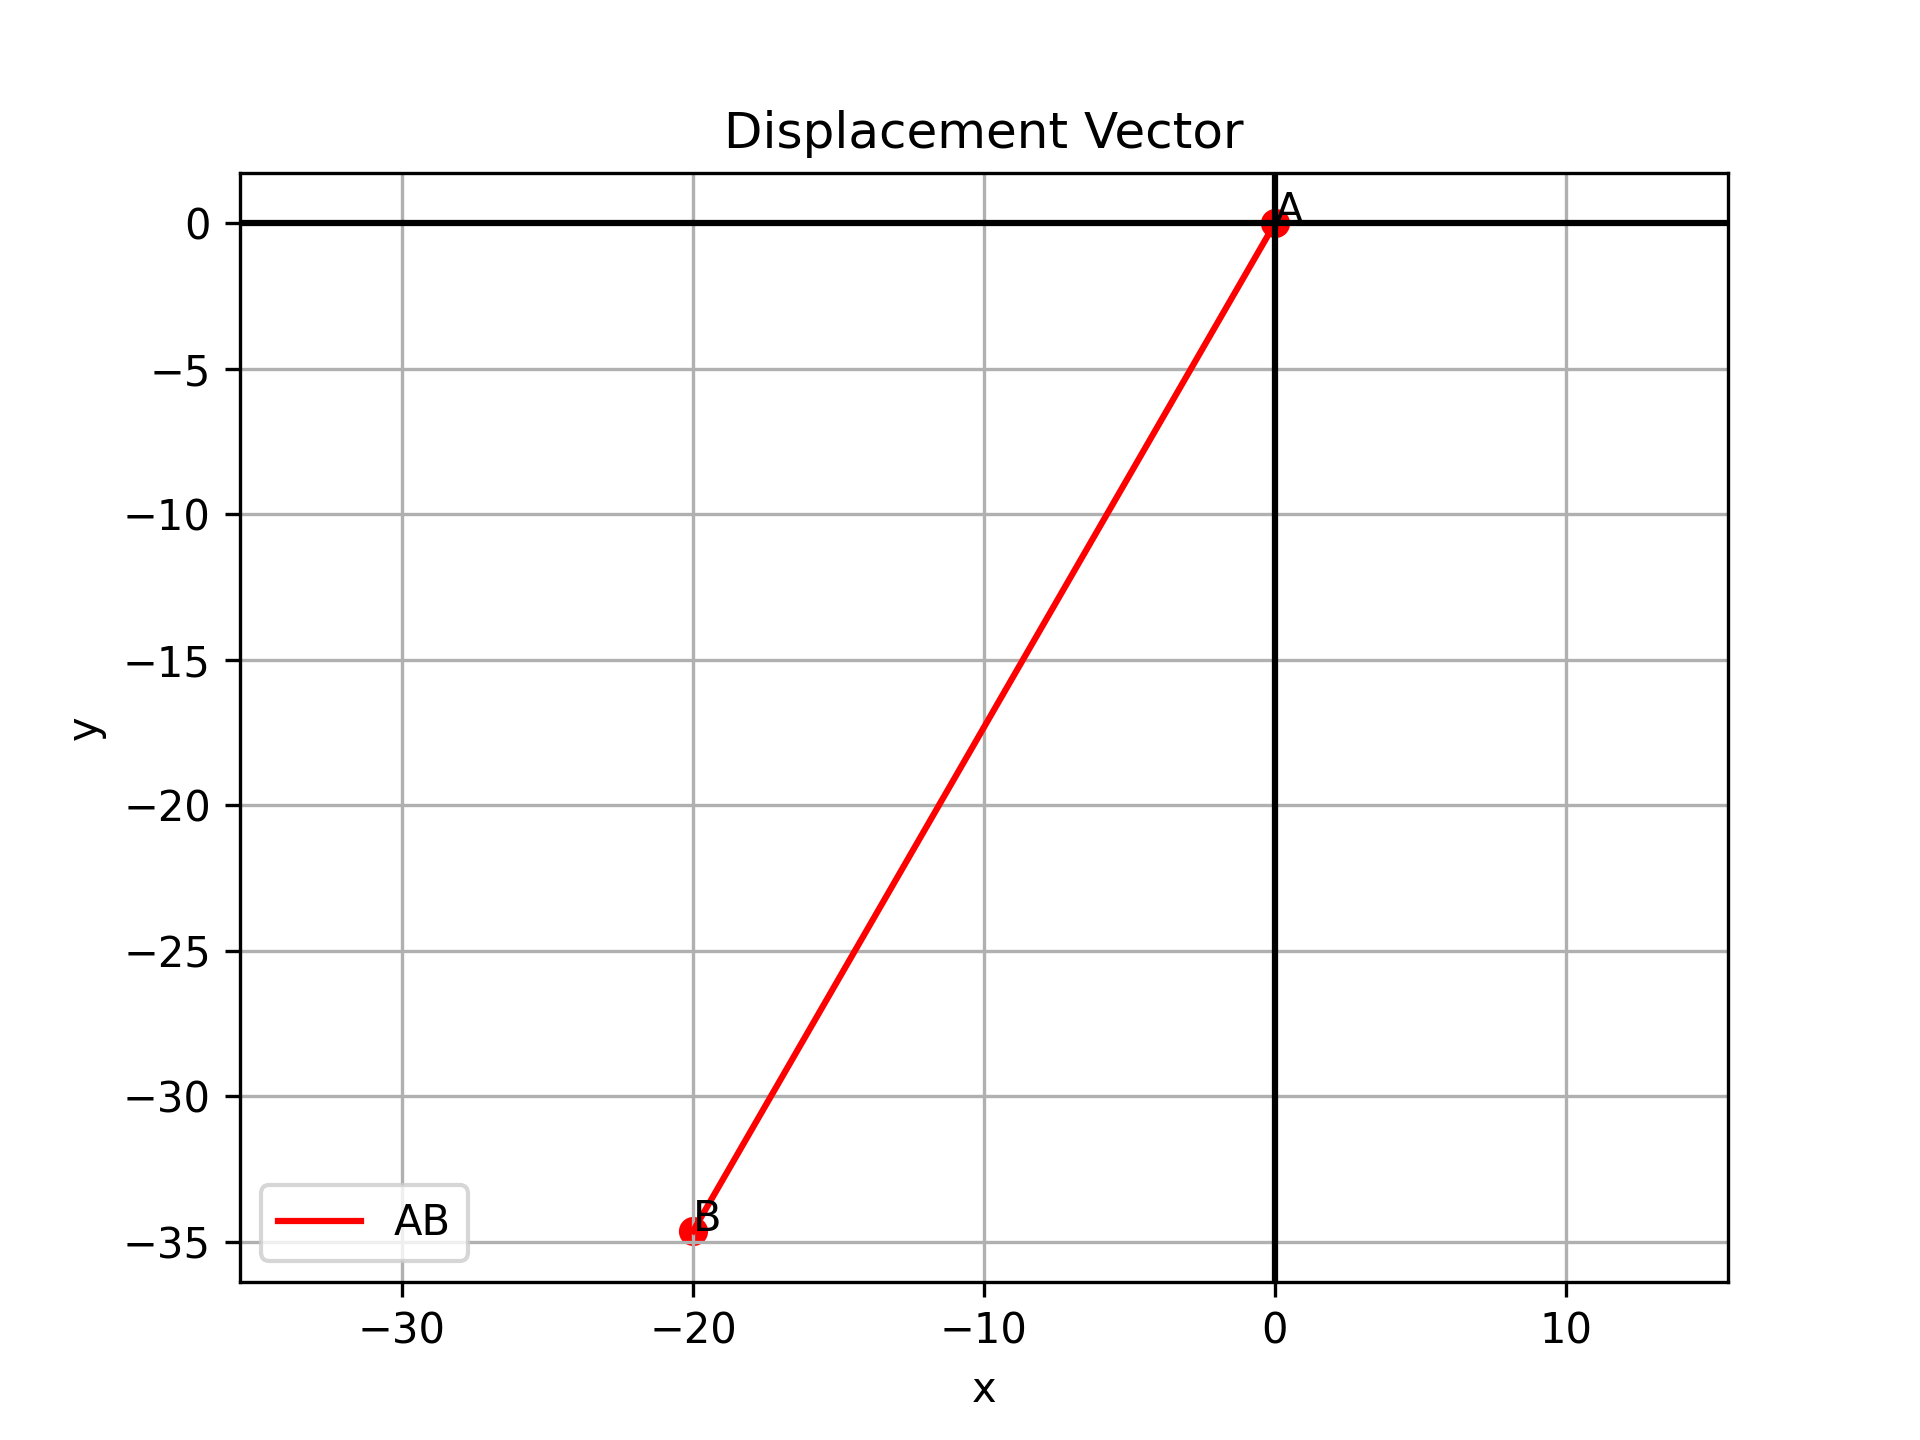
\includegraphics[width=0.65\linewidth]{figs/fig.png}
    \caption{Displacement vector: 40 km, $30^{\circ}$ west of south}
\end{figure}

\end{document}
